\documentclass[10pt,a4paper, enlgish, spanish]{article}

\usepackage{color}     % para snipets de codigo coloreados
\usepackage{amsmath}
\usepackage{amsfonts}
\usepackage[utf8]{inputenc}
\usepackage[T1]{fontenc}
\usepackage{geometry}
 \geometry{
    a4paper,
    total={210mm,297mm},
    left=5mm,
    right=5mm,
    top=15mm,
    bottom=15mm
 }

\usepackage{dependencies/caratula,dependencies/aed2-symb,dependencies/aed2-itef,dependencies/aed2-tad, dependencies/aed2-helper}
\usepackage[spanish]{babel}
\usepackage{fancyhdr}
\usepackage{algorithm2e}
\usepackage{algpseudocode}
\usepackage{listings}
\usepackage{xcolor}
\usepackage{pdfpages} 
\usepackage{fancybox}  % para el sbox de los snipets de codigo
\usepackage{graphicx}

\usepackage{caption}
\usepackage{subcaption}
\usepackage{float}
\usepackage{lastpage}
\usepackage{afterpage}


% definiciones

\newtheorem{theorem}{Teorema}[section]
\newtheorem{lemma}[theorem]{Lema}
\newtheorem{proposition}[theorem]{Proposici\'on}
\newtheorem{corollary}[theorem]{Corolario}

\newcommand{\Var}{\textbf{var }}
\newcommand{\True}{\textbf{true }}
\newcommand{\False}{\textbf{false }}
\newcommand{\Break}{\textbf{break }}

\newenvironment{proof}[1][Demostraci\'on]{\begin{trivlist}
\item[\hskip \labelsep {\bfseries #1}]}{\end{trivlist}}
\newenvironment{definition}[1][Definici\'on]{\begin{trivlist}
\item[\hskip \labelsep {\bfseries #1}]}{\end{trivlist}}
\newenvironment{example}[1][Ejemplo]{\begin{trivlist}
\item[\hskip \labelsep {\bfseries #1}]}{\end{trivlist}}
\newenvironment{remark}[1][Observaci\'on]{\begin{trivlist}
\item[\hskip \labelsep {\bfseries #1}]}{\end{trivlist}}

\definecolor{litegrey}{gray}{0.94}

\newenvironment{codesnippet}{%
	\begin{Sbox}\begin{minipage}{\textwidth}\sffamily\small}%
	{\end{minipage}\end{Sbox}%
		\begin{center}%
		\vspace{-0.4cm}\colorbox{litegrey}{\TheSbox}\end{center}\vspace{0.3cm}}

\lstset{frame=tb,
	  language=Java,
	  aboveskip=3mm,
	  belowskip=3mm,
	  showstringspaces=false,
	  columns=flexible,
	  basicstyle={\scriptsize\ttfamily},
	  numberstyle=\tiny\color{gray},
	  keywordstyle=\color{blue},
	  commentstyle=\color{green},
	  stringstyle=\color{red},
	  breaklines=true,
	  breakatwhitespace=true,
	  tabsize=3,
	  numbers=left,
	  numbersep=15pt,
	  numberfirstline = false
	}


\begin{document}

% **************************************************************************
%
%  Package 'caratula', version 0.2 (para componer caratulas de TPs del DC).
%
%  En caso de dudas, problemas o sugerencias sobre este package escribir a
%  Nico Rosner (nrosner arroba dc.uba.ar).
%
% **************************************************************************



% ----- Informacion sobre el package para el sistema -----------------------

\NeedsTeXFormat{LaTeX2e}
\ProvidesPackage{caratula}[2003/4/13 v0.1 Para componer caratulas de TPs del DC]


% ----- Imprimir un mensajito al procesar un .tex que use este package -----

\typeout{Cargando package 'caratula' v0.2 (21/4/2003)}


% ----- Algunas variables --------------------------------------------------

\let\Materia\relax
\let\Submateria\relax
\let\Titulo\relax
\let\Subtitulo\relax
\let\Grupo\relax


% ----- Comandos para que el usuario defina las variables ------------------

\def\materia#1{\def\Materia{#1}}
\def\submateria#1{\def\Submateria{#1}}
\def\titulo#1{\def\Titulo{#1}}
\def\subtitulo#1{\def\Subtitulo{#1}}
\def\grupo#1{\def\Grupo{#1}}


% ----- Token list para los integrantes ------------------------------------

\newtoks\intlist\intlist={}


% ----- Comando para que el usuario agregue integrantes

\def\integrante#1#2#3{\intlist=\expandafter{\the\intlist
    \rule{0pt}{1.2em}#1&#2&\tt #3\\[0.2em]}}


% ----- Macro para generar la tabla de integrantes -------------------------

\def\tablaints{%
    \begin{tabular}{|l@{\hspace{4ex}}c@{\hspace{4ex}}l|}
        \hline
        \rule{0pt}{1.2em}Integrante & LU & Correo electr\'onico\\[0.2em]
        \hline
        \the\intlist
        \hline
    \end{tabular}}

% ----- Macro para generar la parte reservada para la c�tedra -------------------------

\def\tablacatedra{%
    \\
    \textbf{Reservado para la cátedra}\par\bigskip
    \begin{tabular}{|c|c|c|}
        \hline
        \rule{0pt}{1.2em}Instancia & Docente & Nota\\[0.2em]
        \hline
        \rule{0pt}{1.2em}Primera entrega & \phantom{mmmmmmmmmmmmmmmmmm} & \phantom{mmmmmm} \\
        \hline
        \rule{0pt}{1.2em}Segunda entrega & & \\
        \hline
    \end{tabular}}

% ----- Codigo para manejo de errores --------------------------------------

\def\se{\let\ifsetuperror\iftrue}
\def\ifsetuperror{%
    \let\ifsetuperror\iffalse
    \ifx\Materia\relax\se\errhelp={Te olvidaste de proveer una \materia{}.}\fi
    \ifx\Titulo\relax\se\errhelp={Te olvidaste de proveer un \titulo{}.}\fi
    \edef\mlist{\the\intlist}\ifx\mlist\empty\se%
    \errhelp={Tenes que proveer al menos un \integrante{nombre}{lu}{email}.}\fi
    \expandafter\ifsetuperror}


% ----- Reemplazamos el comando \maketitle de LaTeX con el nuestro ---------

\def\maketitle{%
    \ifsetuperror\errmessage{Faltan datos de la caratula! Ingresar 'h' para mas informacion.}\fi
    \thispagestyle{empty}
    \begin{center}
    \vspace*{\stretch{2}}
    {\LARGE\textbf{\Materia}}\\[1em]
    \ifx\Submateria\relax\else{\Large \Submateria}\\[0.5em]\fi
    \par\vspace{\stretch{1}}
    {\large Departamento de Computaci\'on}\\[0.5em]
    {\large Facultad de Ciencias Exactas y Naturales}\\[0.5em]
    {\large Universidad de Buenos Aires}
    \par\vspace{\stretch{3}}
    {\Large \textbf{\Titulo}}\\[0.8em]
    {\Large \Subtitulo}
    \par\vspace{\stretch{3}}
    \ifx\Grupo\relax\else\textbf{\Grupo}\par\bigskip\fi
    \tablaints
    \vspace*{\stretch{3}}
    \medskip
    \\
    Utililizaremos un clasificador de K-Vecinos más cercanos para etiquetar imágenes de dígitos manuscritos. Con el fin de mejorar su comportamiento se calcularán los autovalores y autovectores más grandes para mediante PCA seleccionar los rasgos más característicos de los dígito en las imágenes. Gracias a métricas como accuracy compararemos el resultado de la aplicación del método con distintos parámetros y conjuntos de entrenamiento usando Cross Validation.
    \\
    \vspace*{\stretch{3}}
    {\bf Palabras claves:} OCR, K nearest neighbours, PCA, Cross Validation.
    \vspace*{\stretch{3}}
    \medskip
    \tablacatedra
    \end{center}
    \vspace*{\stretch{3}}
    \newpage
    }
\newpage

\tableofcontents
\newpage

\section{Introducción}

\newpage

\section{Desarrollo}


\newpage

\section{Resultados y discusión}

\newpage

\section{Conclusión}


\newpage

\section{Apéndice} \label{cap:apendice}

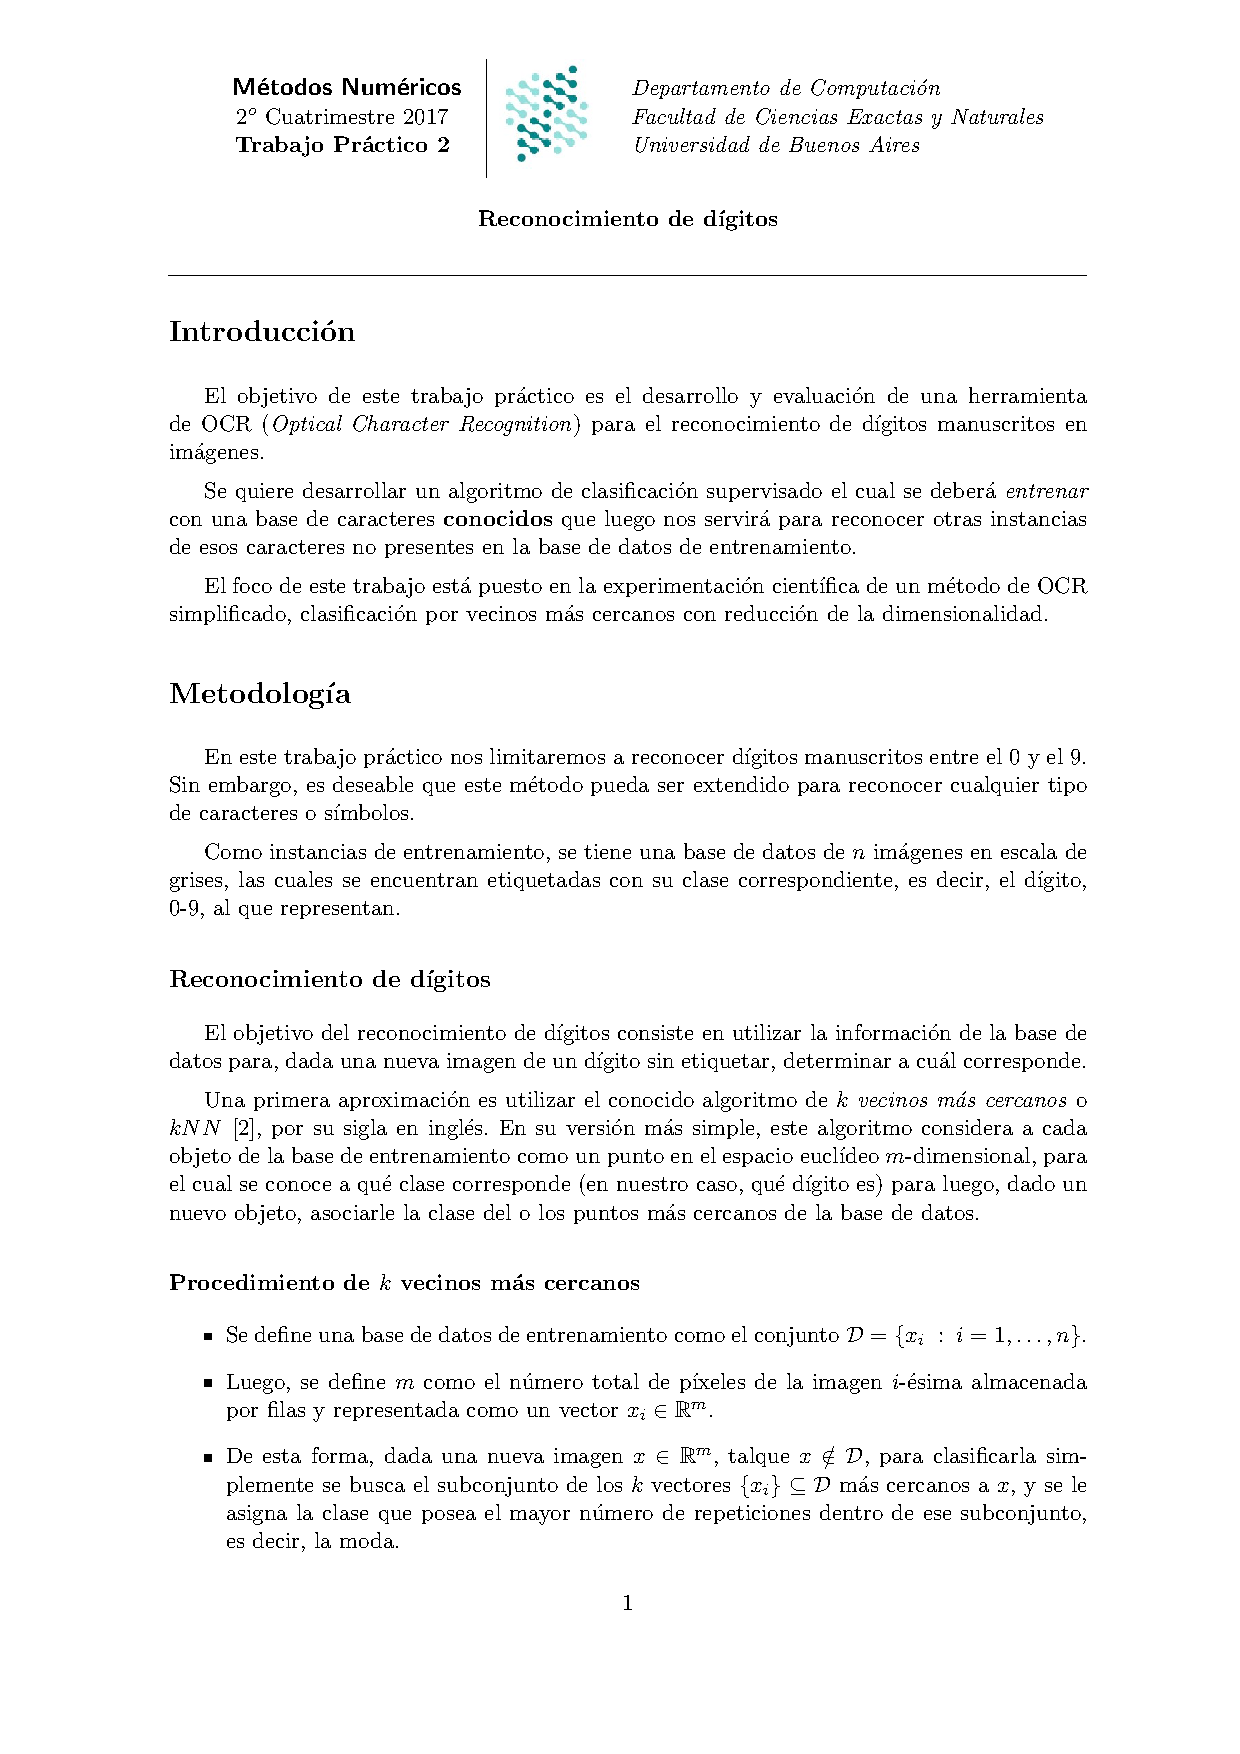
\includepdf[pages=-]{../enunciado/tp2.pdf}

\newpage

\section{Referencias}

 
\begin{thebibliography}{9}


\end{thebibliography}



%\input{others/comentarios}

\end{document}
